\chapter{Estado del Arte}
\label{sec:estadodelarte}

En calidad de abordar la búsqueda de precisión decimétrica en sistemas de posicionamiento, se ha realizado un breve recorrido por la literatura para clasificar aquellos trabajos que se consideran relevantes para el desarrollo de la presente investigación.\\ 

Producto de la revisión de los trabajos desarrollados durante las últimas dos décadas y relacionados con temas de interés para le presente investigación, se considera la clasificación de los mismos en 3 grandes grupos. \\

En el primer grupo a considerar, se encuentran los trabajos relacionados con el modelado matemático y representación de fenómenos relacionados con el comportamiento de la ionosfera, troposfera durante el viaje de la señal desde el satélite al receptor, así como el planteamiento de modelos corrección y predicción de orbita de satélites y/o errores por efectos de reflexión y difracción, que tienen incidencia el nivel de precisión en tareas de localización y posicionamiento. \\

Un segundo grupo, es el orientado a la mejora y desarrollo de aplicaciones GNSS apoyado en la integración de tecnologías emergentes y la tecnología GNSS, para aplicaciones civiles, comerciales y científicas, como son los casos de integración de unidades de medición inercial (IMU) con GPS, Indoor-GPS, Outdoor-GPS, etc, en sistemas de transporte inteligente (ITS), medición del desplazamiento de capas tectónicas, medición de nivel de cauce en ríos y lagos, entre otros.\\

Dentro de este grupo, los estudios relacionados van desde el estudio patrones de movimiento de la población dentro de mercados ambulantes \cite{Tsang_2011}, atractivos turísticos y zonas de reserva natural \cite{Meijles_2014}, \cite{Orellana_2012}; hasta el desarrollo de un sistemas de posicionamiento cooperativos para sistemas de trasporte inteligente (ITS) dentro de ambientes urbanos \cite{Tang_2014}.\\

Finalmente una publicación que presenta una interesante visión del futuro de la tierra basada el uso de Internet de la cosas (IOT) \cite{Li_2014}. Se propone una completa infraestructura apoyada en dispositivos móviles, que trabajan como sensores y entregan información a un servicio web encargado de generar modelos de información locales y globales. Con la información presentada mediante modelos de información 3D, tendrían información útil para la prevención de desastres naturales, pronostico del clima y estudios de fenómenos geológicos.\\  

Todas las áreas presentadas en esta clasificación tienen una característica u objetivo en común y es que, con el aporte de cada uno de ellos lo que se busca es tener un posicionamiento de precisión. 

\begin{figure}[h]
	\centering
    \subfigure[Palabras Claves.]{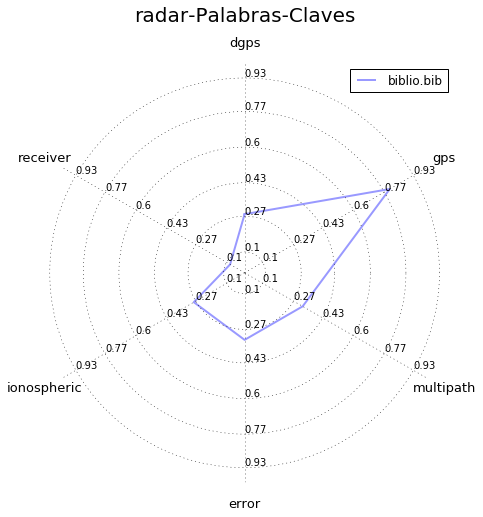
\includegraphics[scale=0.4]{Imagenes/ReporteBiblio/radar-Palabras-Claves.png}}
    \subfigure[Tipos de Documento.]{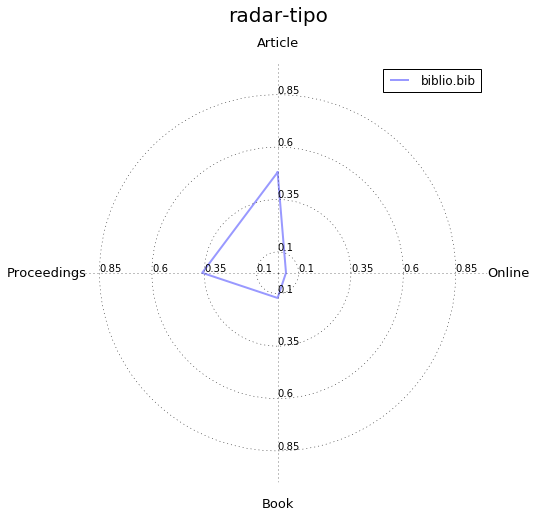
\includegraphics[scale=0.4]{Imagenes/ReporteBiblio/radar-tipo.png}}
	\caption{Extracción de información desde Estado del arte.}
	\label{fig:EstadoArte1}
\end{figure}

Los valores presentados en la Figura \ref{fig:EstadoArte1}, corresponden a valores porcentuales producto de la revisión de un total de 30 documentos, para llevar a cabo el planteamiento de la presente propuesta.\\

En listado de palabras presentado en la Figura \ref{fig:Relativewords}, es producto de la asociación de la palabras claves encontradas en cada articulo revisado, que dan idea de los temas que pueden estar relacionados con el objeto de esta investigación y que permiten tener una idea del contexto y trabajos relacionados con la misma. 

\begin{figure}[h]
	\centering
    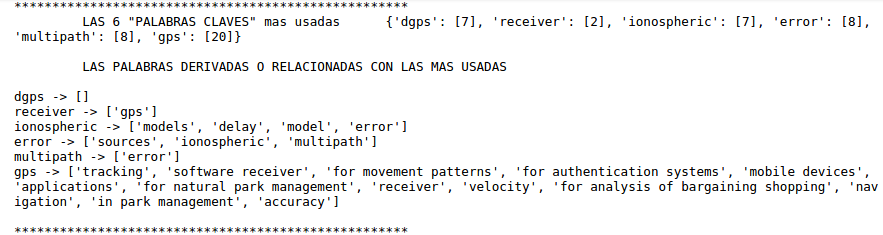
\includegraphics[scale=0.5]{Imagenes/ReporteBiblio/Relative_words.png}
	\caption{Palabras derivadas o relacionadas con las palabras claves de los artículos revizados.}
	\label{fig:Relativewords}
\end{figure}




